% arara: pdflatex: { shell: true, draft: true }
% arara: makeglossaries
% arara: biber
% arara: pdflatex: { shell: true, synctex: true }
% arara: pdflatex: { shell: true, synctex: true }

\documentclass[12pt,DIV14,BCOR10mm,a4paper,parskip=half-,headsepline,headinclude,english,ngerman,bibliography=totocnumbered]{scrreprt}

\usepackage{hshhelper_base}

%%%%%%%%%%%%%%%%%%%%%%%%%%%%%%%%%%%%%%%%%%%%%%%%%%%%%%%%%%%%%%%%%%%%%%%%%%
\begin{document}    % hier gehts los
  \thispagestyle{empty} % Titelseite

\includegraphics[width=0.2\textwidth]{Wortmarke_WI_schwarz}

   {  ~ \sffamily
  \vfill
  {\Huge\bfseries Architekturbeschreibung}
  \bigskip

  {\Large
  Dennis Grabowski, Julius Zint, Philip Matesanz, Torben Voltmer \\[2ex]
  Masterprojekt \enquote{Entwicklung und Analyse einer sicheren \\Web-Anwendung} \\
  Wintersemester 18/19
 \\[5ex]
   \today }
}
 \vfill

  ~ \hfill
  
\includegraphics[height=0.3\paperheight]{H_WI_Pantone1665}

\vspace*{-3cm}

\tableofcontents  % Inhaltsverzeichnis

\chapter{Architekturaufbau}
\section{Klassendiagramm}

Das in Abbildung \ref{architecture:class_diagram} dargestellte Architekturdiagramm verzichtet zugunsten der Über\-sichtlichkeit auf die Abhängig\-keiten zwischen den Klassen. Es dient lediglich zur Veranschaulichung der Top-Level-Architektur und zur Illustration der wichtigsten Klassen. Der Zusammenhang der farblich abgetrennten Gruppierungen wird zusätzlich textuell erklärt.

% ggf. explizit Farben nennen?
Zu jedem Controller gibt es einen Manager in der Domänenlogik.
Dieser enthält jegliche Logik zur Abarbeitung der Anfrage und liefert auftretende Fehler über eine Exception zurück. Ein Datenbankzugriff erfolgt somit niemals von einem Controller, sondern immer aus dem zugehörigen Manager.
Beim Sessionmanager handelt es sich um einen Spezialfall, da das Session-Konzept ein integraler Bestandteil der Anwendung ist, da die Prüfung auf vorhandene Authentifizierung Grundlage aller Aktionen ist\footnote{Siehe Anforderungsbeschreibung 4.2: Sämtliche Funktionen von HsH-Helfer sind nur angemeldeten Benutzern zugänglich.}.

Das Gleiche gilt für das \texttt{PasswordSecurityModule}, welches beim Login, Erstellen eines Nutzers sowie dem \enquote{Passwort zurücksetzen} benötigt wird, da in ihr alle Passwort-Operationen gekapselt sind.
Daher wurden diese beiden Klassen unter \enquote{Cross-Cutting-Concerns} zusammengefasst.
Zugriffe auf diese Klassen können sowohl von Controllern als auch von Managern in der Domänenlogik erfolgen. \par
Im Folgenden geben Sequenzdiagramme weitere Einsicht in das Zusammenspiel dieser Klassen.

Die Klassen, die in der zweiten Iteration dazu gekommen sind, können der Abbildung \ref{architecture:class_diagram2} entnommen werden.
Der Aufbau des zweiten Klassendiagramm gleicht dem Aufbau des ersten.

\section{Sequenzdiagram: Benutzer erstellen}

Beim Anlegen eines neuen Benutzers wird zuerst durch ein HTTP GET das Formular angefragt.
Dies ist notwendig um ein gültiges CSRF-Token zu erhalten, welches beim anschließenden HTTP POST mitgeliefert werden muss. Auch hier wird bereits, wie aus dem Sequenzdiagramm \ref{architecture:createuserseq_diagram} ersichtlich, überprüft ob der anfragende User authentisiert ist.
Ist das der Fall, wird ein HTML Formular zurückgeliefert, die ausgefüllt und durch eine weitere Anfrage wieder an den Server geschickt wird.
Hier wird zuerst über die in Play integrierte Möglichkeit der Annotations eine erste Validierung der Eingaben vorgenommen.
Somit werden Eingaben mit nicht unterstützten Zeichen oder ungültiger Länge früh herausgefiltert und dem Benutzer durch Anzeigen von Fehlermeldungen direkt am Eingabefeld mitgeteilt.
Sind alle Eingaben korrekt, wird der Aufruf an den Manager weitergeleitet.
Dieser befragt zuerst die Policy, ob der authentisierte Benutzer autorisiert ist, einen neuen Benutzer anzulegen.
Nach erfolgreicher Prüfung generiert er ein neues Passwort, hashed es und legt in einer Transaktion einen neuen Benutzer an.
Das Klartext-Passwort wird zurückgegeben und dem Administrator angezeigt, um dies dem neuen Benutzer zukommen zu lassen.

\section{Sequenzdiagram: Login}

Das Login-Sequenzdiagramm \ref{architecture:loginseq_diagram} zeigt den Fall, dass der Benutzer bereits mehrfach das Passwort falsch eingegeben hat und ein Captcha lösen muss. In der Antwort, die auf die erste GET Anfrage folgt, sind sowohl das CSRF-Token als auch das HTML zum Lösen des Captchas enthalten. In der darauffolgenden POST Anfrage werden die Captcha-Information, sowie der Benutzername und das Passwort aus dem Formular mitgeliefert. Bei beiden Anfragen wird noch sichergestellt, dass der Benutzer nicht bereits eine gültige Session besitzt, um mehrfache Logins zu vermeiden. Die Eingaben werden, wie auch schon bei Nutzer erstellen, zuerst durch Annotations validiert und anschließend an den \texttt{LoginManager} weitergereicht. Diese berechnet unabhängig von der Existenz des Nutzerkontos den Hash des Klartext-Passworts und vergleicht diesen mit dem Hash, der zum Benutzerkonto abgespeichert wurde, falls vorhanden. Anschließend wird die Login-Firewall befragt, ob es Unstimmigkeiten für diesen Benutzer oder die anfragende IP-Adresse gibt. In dem hier vorgestellten Fall liefert diese \texttt{Verify} zurück, was bedeutet, dass dieser Benutzer ein Captcha lösen muss. Anschließend wird überprüft, ob es erfolgreich gelöst wurde und dann wird beim \texttt{SessionManager} durch den Aufruf von \texttt{startNewSession} eine neue Session erzeugt. Damit wurde der Login erfolgreich abgeschlossen.


\section{Dateiaustausch}
Alle Dateien, die von Benutzern hochgeladen werden, werden in der Datenbank als \texttt{BLOB} gespeichert. So können konsistente Zustände mittels Transaktionen sichergestellt werden. Außerdem ist HsHelper dadurch unabhängiger vom Dateisystem, das auf dem Host-System verwendet wird.

Dadurch, dass wir Java-seitig ein Byte-Array (\texttt{byte[]}) als Datentyp für den Dateiinhalt verwenden, besteht eine Obergrenze von $2^{31}$ Bytes (2,147 Gigabyte) \footnote{Siehe 4.2.1 Integral Types and Values \url{https://docs.oracle.com/javase/specs/jls/se8/html/jls-4.html\#jls-4.2}} für die Dateigröße, da die Länge sowie der Index eines Byte-Arrays als Integer verwaltet wird.

Um die Umgehung des Speicherplatzlimits durch Ausnutzung des Kommentarfeldes und Dateinamens zu verhindern, zählen sowohl der Datei-Inhalt, als auch Dateiname und Kommentar zum Speicherplatz, den eine Datei belegt.
Dabei nehmen wir an, dass jedes Zeichen des Dateinamens und des Kommentars jeweils 1 Byte Speicherplatz verbraucht und machen keine Annahmen über die verwendete Zeichenkodierung.
Somit werden auch obskure Unicodezeichen dem Nutzer mit jeweils 1 Byte in Rechnung gestellt.
Wir halten dies für eine faire Annahme, vor allem unter Berücksichtigung eines typischen Nutzers, der die Unterschiede von Unicode zu anderen Zeichenkodierungen nicht kennt.

Beim Herunterladen von Dateien wird der Content-Disposition Modus auf \texttt{attachment} und Content-Type auf \texttt{application/octet-stream} gesetzt. So wird erzwungen, dass der Browser immer den \enquote{Speichern}-Dialog anzeigt statt die Datei direkt (im Browser) darzustellen\footnote{Das wäre zum Beispiel bei Textdateien, Bildern und PDFs möglich.}.

\section{Logging}

Aufgrund der Bedrohung \textit{T11: Abstreitbarkeit illegaler Handlungen} wurde ein Logging implementiert, mit dem sichergestellt wird, dass genau das nicht passieren kann.

Im Zuge dessen wurden 2 verschiedene Logs mithilfe der Bibliothek \enquote{Logback}, die Play standardmäßig inkludiert, implementiert.
Einmal ein generelles Zugriffslog, in welchem jegliche Zugriffe auf unsere Seite dokumentiert werden, und ein domänenspezifisches Log, in dem spezielle Loggingausgaben für die einzelnen, vorhandenen Aktionen persistiert werden.
Das Zugriffslog wird in der Datei \texttt{logs/access.log} unter Beachtung eines angepassten \textit{Apache Log Format} persistiert.
Das Format ist wie folgt aufgebaut:

\texttt{[Timestamp] - IPAdresse - Username "HTTPVerb HTTPPath"}

Für den Fall, dass kein Username vorhanden ist, beispielsweise ein Angreifer oder Endpoints, die auch ohne Authentifizierung erreichbar sind, wird \enquote{unauthorized user} geloggt.

Im domänenspezifischen Log, dem \texttt{logs/application.log}, wird nach dem vorgegebenem Format von \enquote{Logback} persistiert.
Dieses sieht wie folgt aus:

\texttt{[Timestamp] - [LogLevel] - from JavaClass in JavaThread\\
domainspecificLogMessage}

Um den Schaden eines Log Poisoning zu mitigieren, loggen wir nur die IDs der einzelnen Entitäten sowie Teile dieser Entitäten, die validiert wurden.
Konkret heißt das, dass wir Benutzername, Gruppenname und Dateiname loggen.
Diese werden nämlich durch die Eingabevalidierung mithilfe eines Regex geprüft, so dass nur erlaubte Zeichen durchkommen.

Um einen weiteren Schutz zu bieten, haben wir Play's Loggerschnittstelle erweitert, so dass wir weitere, potentiell gefährliche Zeichen aus einer zu loggenden Ausgabe herausfiltern können.
Bisher filtern wir nur Zeilenumbrüche heraus, damit ein Angreifer nicht in der Lage ist, ein fiktives Logstatement zu injizieren, um beispielsweise einem anderen Nutzer eine illegale Aktion unterzujubeln.

Generell loggen wir folgende Aktionen:
\begin{itemize}
	\item Erstellen von Nutzern, Gruppen sowie Dateien
	\item Löschen von Nutzern, Gruppen sowie Dateien
	\item Änderungen an Dateikommentar, -inhalt und -Berechtigungen
	\item Änderungen an der Mitgliederliste einer Gruppe
	\item Versuch, bestehende Einschränkungen zu brechen (Speicherplatzlimit versucht zu überschreiten, Gruppenname existiert bereits...)
\end{itemize}

\chapter{Kryptografisch relevante Informationen}
Folgender Abschnitt enthält gesammelte Informationen über die kryptographischen Algorithmen, die im HsH-Helper Anwendung finden. Die für die Algorithmen benötigten Geheimnisse und deren Verwaltung wird ebenfalls hier dokumentiert, da die Sicherheit von der Geheimhaltung dieser abhängt.

\section{Passwörter}
Die Passwörter, die Benutzer verwenden um sich beim HsH-Helper zu authentisieren, werden grundsätzlich nur als Hash persistiert. Konkret wird die Hashfunktion bcrypt zum Hashen der Passwörter verwendet.

Um ein Passwort mit bcrypt zu hashen, muss zunächst ein Salt generiert werden. Neben dem Salt und dem gehashten Passwort wird bei bcrypt außerdem noch die bcyrpt Version und die Anzahl der Runden gespeichert. Über die Anzahl der Runden kann die Laufzeit, die bcrypt benötigt, um ein Passwort zu hashen, beeinflusst werden.

Die verwendete Bibliothek ist jBCrypt von mindrot.org (org.mindrot.jbcrypt) in der Version 0.4. Sie verwendet intern die Java Klasse SecureRandom als CSPRNG.

Auch zur Generierung der initialen (und temporären) Benutzer-Passwörter beim Anlegen eines neuen Benutzerkontos wird SecureRandom als Basis verwendet. Dafür zuständig ist die Klasse \texttt{PasswordGenerator}. Die generierten Passwörter können die Zeichen \texttt{a-z}, \texttt{A-Z}, \texttt{0-9} und die Sonderzeichen \texttt{!\%?\#-\_*+} enthalten.

\section{CSRF-Tokens}
Die CSRF-Tokens, die das Play Framework generiert, bestehen aus 3 Teilen:
\begin{enumerate}
% SecureRandom ist cSprng.
\item Einem Token, dass für jede Session mit der Java Klasse SecureRandom als CSPRNG generiert wird.
\item Einer auf der Systemzeit basierendem Nonce, dass für jeden Request generiert wird.
\item Einer auf HMAC-SHA1 basierenden Signatur des Tokens und der Nonce.
\end{enumerate}

Beim Starten einer Play-Session wird ein CSRF-Token in das Session Cookie geschrieben. Dieses CSRF-Token ändert sich während einer Play-Session nie. Für jedes Formular wird ein eigenes CSRF-Token generiert, dass sich innerhalb einer Play-Session nur durch die Nonce (und damit auch der Signatur) unterscheidet. Durch Vergleichen des Tokens aus dem CSRF-Token der Play-Session und des Tokens aus dem CSRF-Token in einem HTTP Request kann die Gültigkeit eines CSRF-Token festgestellt werden.


\section{Play Cookies}
\label{play:cookies}
Das Play Framework nutzt zur Persistierung eines Cookies in dem Client-Browser das \enquote{\gls{jwt}}-Format.
Ein \gls{jwt} besteht aus 3 Teilen: einem Header, einer Payload sowie einer Signatur, siehe \ref{jwtformat}.
Jeder dieser Teile ist ein namenloses JSON-Objekt. \\
Innerhalb des Headers ist gelistet, welcher Algorithmus genutzt wurde, um das JWT zu signieren.
Die Payload ist ein einfaches JSON-Objekt, in welchem Daten gespeichert werden können, die zu signieren sind.
Diese Daten werden innerhalb des JWT-Formats als \enquote{Claims} bezeichnet.
Zusätzlich werden innerhalb dieser Payload persistiert, zu welchem Zeitpunkt das JWT erstellt wurde, ab welchem Zeitpunkt es gültig ist und wann es ausläuft.
Für die Signatur werden Header sowie Payload durch \enquote{base64url} kodiert und dann zusammen mit einem Punkt als Trennelement konkateniert. Die dadurch entstehende Zeichenkette wird zusammen mit einem geheimen Schlüssel an den kryptografischen Signatur-Algorithmus weitergegeben, der zuvor im Header genannt wird.
Play verwendet standardmäßig zur Signierung den HMAC-SHA256 Algorithmus.
Dadurch kann die Integrität der Claims geprüft werden und zeitgleich können sie authentifiziert werden. \\
Um das JWT nun bilden zu können, werden alle 3 Teile durch \enquote{base64url} seperat kodiert und durch einen Punkt getrennt und konkateniert: \texttt{encodeBase64Url(header) + '.' + encodeBase64Url(payload) + '.' + encodeBase64Url(signature)}.
\par
Bei Werkseinstellungen verwendet Play ein Cookie namens \textit{PLAY\_SESSION}, in dessen Payload ein zusätzliches JSON-Objekt namens \texttt{data} sowie die Zeitstempel für Erstellungsdatum sowie Beginn der Gültigkeit gespeichert sind.
In dem JSON-Objekt \texttt{data} persistiert Play das CSRF-Token, erlaubt einer Applikation allerdings dort auch Daten abzulegen.
Wie später zu sehen ist, baut unser Session-Konzept darauf auf.

Neben dem Session Cookie gibt es noch das Flash Cookie \textit{PLAY\_FLASH}, was allerdings in der aktuellen Iteration keinerlei Anwendung findet. Der Error-Handling-Code verwendet zwar den Flash-Scope um Fehlermeldungen über eine Klassengrenze hinweg verfügbar zu machen, diese Daten werden aber innerhalb einer Anfrage direkt wieder gelesen und landen somit niemals beim Client.

Die Dokumentation von Play vermerkt, dass das Flash Cookie nicht signiert wird:
\blockquote{
The Flash scope works exactly like the Session, but with two differences: \\
\textbf{-} data are kept for only one request, \\
\textbf{-} the Flash cookie is not signed, making it possible for the user to modify it. \autocite{JavaPlayFlashDocu}
}
Dies hat sich allerdings bei einem Test als falsch herausgestellt. Das Flash Cookie wird in unserer Anwendung sowohl signiert als auch validiert, wenn es vom Client bei einer weiteren Anfrage wieder an den Server geschickt wird.

\section{Schlüsselmanagement}
Für das System sind mehrere Schlüssel und Zugangsdaten notwendig:

\begin{itemize}
	\item Der private Schlüssel zum Signieren der Play Cookies
	\item Der private Schlüssel für reCAPTCHA
	\item Der öffentliche Schlüssel für reCAPTCHA
	\item Zugangsdaten für den E-Mail Server
	\item Zugangsdaten für die Datenbank
\end{itemize}

Der öffentliche reCAPTCHA-Schlüssel wird benötigt, um das reCAPTCHA einbinden zu können und wird vom Client an Google übertragen. Löst der Client ein Captcha korrekt, erhält er von Google eine Nonce, die er an uns weiterleitet. Diese wird von unserem Server in Verbindung mit dem Private Key an Google geschickt. Google teilt uns dann mit, ob diese Nonce valide ist.

Der öffentliche Schlüssel ist fest mit \enquote{unserer Domain} (localhost) verbunden. Das heißt, dass der Captcha-Code nicht auf einer anderen Domain eingebunden werden kann, um Noncess zu erzeugen.

Daher werden alle Schlüssel sowie Zugangsdaten in der \texttt{secrets.conf} Datei auf jedem Entwicklungsrechner der Teammitglieder persistiert, welche nicht versioniert wird. Die \texttt{application.conf} bindet diese Datei mit dem \texttt{include}-Statement ein und somit werden die Schlüssel in der Anwendung verwendet. Dies hat den offensichtlichen Vorteil das Zugangsdaten nicht im Repository einsichtlich sind, aber Anwendungseinstellungen jedoch schon.

\chapter{Sicherheitsmaßnahmen}

\section{Login-Firewall}
Der Login einer Web-Anwendung ist potentiell anfällig für Brute-Force-Angriffe, die darauf abzielen, eine valide Kombination aus Benutzername und Passwort zu finden. Aus diesem Grund muss die Anwendung fehlerhafte Zugriffsversuche protokollieren und wenn eine Häufung selbiger auftritt, Maßnahmen ergreifen, um den Angriff zu verlangsamen oder gar zu stoppen. Die zu ergreifende Maßnahme sollte so gewählt werden, dass sie nicht selbst einen Angriffsvektor darstellt, wie z.B. das vollständige Sperren eines Accounts nach N falschen Logins - man könnte so legitime Nutzer vorsätzlich an der Benutzung der Anwendung hindern (Denial of Service).

Aus diesem Grund verfügt unsere Anwendung über eine Komponente\footnote{policy.ext.loginFirewall}, die falsche Logins protokolliert und eine der folgenden Maßnahmen ergreift:

\begin{itemize}
\item Spezifischen Benutzer-Account in Captcha-Mode versetzen
\item Spezifische IP-Adresse in Captcha-Mode versetzen
\item Spezifische IP-Adresse von Logins ausschließen
\end{itemize}

Beim Captcha-Mode handelt es sich um eine Maßnahme, bei der ein Login lediglich möglich ist, wenn zugleich ein Google reCAPTCHA gelöst wird. Eine vollständige Sperrung eines Accounts findet durch unsere Firewall so nicht statt. Es wurde die Annahme getroffen, dass das automatisierte Lösen der reCAPTCHAs zu aufwändig \& teuer für einen Angreifer ist. Zugleich ist das \enquote{unnötige} Lösen eines Captchas für das Opfer ein vertretbares Hindernis.

Lediglich IP-Addressen werden als schärfste Maßnahme vollständig von Logins ausgeschlossen. Sofern ein Angreifer nicht die gleiche IP-Adresse wie sein Opfer verwendet, kann er sich höchstens selbst vom Dienst ausschließen. Sollte eine Situation vorliegen, bei der sich eine Vielzahl an Nutzern eine IP-Adresse teilt, besteht die Möglichkeit, diese von der vollständigen Sperre auszunehmen.

Die interne Datenstruktur der Login Firewall ist darauf optimiert, möglichst wenig Speicher zu verwenden und nutzt Buckets, um aggregierte Informationen über Login-Versuche zu speichern. Die Buckets bilden ein fixes Zeitinterval ab. Führt ein Angreifer eine Million fehlerhafte Logins in zehn Minuten durch, werden lediglich zwei Datenbank-Einträge erstellt: Einen mit Bezug auf den betroffenen Nutzer-Account und einen mit Bezug auf die IP des Angreifers. Beide Einträge verfügen über eine Zählvariable, die jeweils die Anzahl der fehlerhaften Logins beinhaltet.

Der Verweis auf den Nutzer-Account findet über die numerische und eindeutige ID statt, über die jeder Account verfügt. Jener Fallgestaltung, bei der ein Login bei einem nicht-existenten Account erfolgt, wurde ebenfalls Rechnung getragen. Hierbei ist es erforderlich, dass die Firewall exakt so funktioniert, wie bei existierenden Accounts, um ein Informationsleck zu verhindern: Würde die erste Maßnahme nie oder anders greifen als bei tatsächlich existenten Accounts, wäre es möglich zu prüfen, ob ein Account beziehungsweise der dazu korrospondierende Benutzername tatsächlich existiert\footnote{Diese Angriffsform nennt man auch \enquote{Side-Channel Attack}}.

Zu diesem Zweck wird bei nicht-existenten Accounts der Benutzername mittels Hashing auf eine \enquote{virtuelle} User-ID gemappt. Die User-ID wird über ein Long repräsentiert, es wird jedoch ausschließlich der positive Zahlenraum verwendet. Vom Username wird der MD5-Hash gebildet, die ersten 8 Byte werden als Long verwendet und gegebenfalls invertiert. Der so resultierende negative Long-Wert wird in diesem Fall als Grundlage für die Protokollierung fehlerhafter Logins verwendet. Dass MD5 kryptografisch bereits längst als geknackt gilt, ist irrelevant. Wir machen uns lediglich die gute Streuung und hohe Geschwindigkeit von MD5 zu eigen.

\section{Session-Konzept}
\label{sessionkonzept}
Integraler Bestandteil unserer Anwendung ist eine Session-Funktionalität. Theoretisch bietet Play bereits eine Implementierung unter Verwendung von JWT mit der es möglich ist, Daten in Form von signierten Cookies im Client-Browser zu speichern (vgl. \ref{play:cookies}). Die Sicherstellung der Authentifizierung ist jedoch für nahezu jede Funktionalität unserer Anwendung von Bedeutung. Aus diesem Grund wurde das Session-Konzept soweit abstrahiert, dass eine Java-Annotation über einer Controller-Klasse oder einzelnen Controller-Methoden ausreicht, um zu garantieren, dass ausschließlich authentifizierte Nutzer auf selbige zugreifen können.

Die Annotation bewirkt, dass der korrospondierende Request \underline{vor} Erreichen der dazugehörigen Controller-Methode abgefangen wird und einer Prüfung unterzogen wird, ob der Absender authentifiziert ist. Ist dies nicht der Fall, wird die weitere Ausführung abgebrochen und der Nutzer auf die Login-Seite weitergeleitet. Ansonsten wird der Request an den entsprechenden Controller weitergereicht.

Zur Umsetzung dieser Funktionalität setzen wir auf dem Session-Konzept von Play auf.
Initialisiert ein Nutzer eine neue Session, so persistieren wir seine IP-Adresse, seine User-ID, das Initialisierungsdatum und eine kryptografisch sicheren \enquote{\gls{uuid}} als Identifikator dieser neuen Session in unserer Datenbank. \linebreak
Um diese Session sicher beim Client speichern zu können, verwenden wir das bereits genannte Cookie \textit{PLAY\_SESSION}.
Innerhalb des Payloads dieses JWT befindet sich ein JSON-Objekt namens \enquote{data} hinterlegt, zu welchem man weitere Applikationsdaten als Schlüssel-Wert-Paare hinzufügen kann.
Das machen wir uns zu eigen und persistieren das Schlüssel-Wert-Paar (\enquote{HsHSession}: \enquote{UUID}), durch welches wir den Nutzer authentisieren können.
Wir verlassen uns daher nicht auf die Existenz dieses Cookies, sondern nutzen dieses nur, um einen signierten Speicher innerhalb des Client-Browsers verwenden zu können.

Die UUID selbst dient als 2nd Layer of Defense: Sollte die JWT-Signatur geknackt werden, muss der Angreifer noch eine in der Datenbank enthaltene UUID erraten. Selbst wenn er diese Hürde meistert, muss er noch die dazugehörige IP-Addresse kennen, sowie über diese auf unsere Anwendung zugreifen können und dies in einem engen Zeitfenster schaffen, da die Lebenszeit einer Session begrenzt ist. Wie lange eine Session gültig ist kann von HsHelper Benutzern eingestellt werden. Die Einstellung wirkt sich auf alles Sessions eines Benutzers aus. Maximal ist eine Session 24 Stunden gültig.

Die Anwendung verfügt über eine Ansicht, die dem Nutzer sämtliche eigene, \enquote{aktive} Sessions anzeigt und ihm die Möglichkeit bietet, diese nach Bedarf einzeln zu entfernen. Ein Logout-Vorgang führt ebenfalls zur Entfernung der korrospondierenden Session. Um eine Vermüllung der Datenbank zu vermeiden, läuft im Hintergrund ein Prozess, der in festen Zeitintervallen Sessions aus der Datenbank entfernt, die \enquote{veraltet} sind, denn wenn der Benutzer sich nicht ausloggt, sondern einfach den Browser schließt, kann unsere Anwendung keine Kenntnis davon erlangen.

\section{Content Security Policy}
Play verwendet standardmäßig eine sehr restriktive Content Security Policy, die XSS-Angriffe maßgeblich erschwert: Inline-Javascript wird vom Client-Browser grundsätzlich blockiert, es ist lediglich möglich, ein externes Script in eine HTML-Seite einzubinden, das jedoch von der gleichen Top-Level-Domain stammen muss. Zugleich muss dieses Script explizit Javascript als Content-Type im HTTP-Header benennen.

Da unsere Anwendung zum jetzigen Zeitpunkt nur mittelbaren Gebrauch von JavaScript macht, haben wir uns dazu entschlossen, die Content Security Policy zu verschärfen: JavaScript wird grundsätzlich nicht mehr ausgeführt, es sei denn, es handelt sich um die JavaScript-Libraries von reCAPTCHA. Zu diesem Zweck haben wir die entsprechenden Quell-URLs auf die Whitelist gesetzt und somit gleichzeitig die Annahme getroffen, dass wir Google als Host-Provider der Bibliotheken vertrauen\footnote{Erforderliche Urls für die CSP Whitelist: \url{https://developers.google.com/recaptcha/docs/faq}}.

Ebenso haben wir uns entschlossen, Browser, die Content Security Policy nicht unterstützen, von unserer Anwendung auszuschließen. Hiervon sind nur hinreichend alte Browser betroffen\footnote{Siehe \textquote{Browser compatibility} \url{https://developer.mozilla.org/en-US/docs/Web/HTTP/CSP}}.

\section{Eingabevalidierung}
Für einige Parameter gibt es festgelegte Constraints, die in allen entsprechenden Dtos verwendet werden. Das sind:

\begin{itemize}
	\item username
	 \begin{itemize}
			\item Maximale Länge: 20
			\item Regex: [a-z][a-z0-9.]+
		\end{itemize}


	\item password
	\begin{itemize}
		\item Maximale Länge: 72 (Beschränkung von bcrypt)
	\end{itemize}

	\item groupname
	\begin{itemize}
		\item Minimale Länge: 3
		\item Maximale Länge: 20
		\item Regex: [a-zA-Z][a-zA-Z0-9.]+
	\end{itemize}


	\item email
	\begin{itemize}
		% TODO: Add footnote to that class
		\item Regex: Siehe Play Implementierung von \texttt{EmailValidator}
	\end{itemize}

	\item filename
	\begin{itemize}
		\item Maximale Länge: 40
		\item Regex: [a-zA-ZäüöÄÜÖß0-9.,\#\%+\&!"':;~-]+
	\end{itemize}

\end{itemize}

\section{Ausgabecodierung}
Die Zeichen, die ein HsHelper Benutzer in das Kommentarfeld einer Datei eintragen kann, unterliegen keiner Beschränkung.
Aus diesem Grund müssen Sonderzeichen maskiert werden. Wenn in Play Daten vom Typ String in einem Template verwendet werden, geschieht die Maskierung der Zeichen automatisch. So wird zum Beispiel der String \texttt{<script>} durch \texttt{\&lt;script\&gt;} ersetzt.

%    public static final int MAX_USERNAME_LENGTH = 20;
%    public static final int MAX_PASSWORD_LENGTH = 100;
%    public static final String USERNAME_REGEX = "[a-z][a-z0-9.]+";


 %   public static final int GROUPNAME_MIN_LENGTH = 3;
 %   public static final int GROUPNAME_MAX_LENGTH = 20;
 %   public static final String GROUPNAME_REGEX = "[a-z][a-z0-9.]+";

\chapter{Implementierte Zusatzfunktionalität}

\section{Nutzer kann mit seinen aktiven Sessions interagieren}

Im Sinne von Ka-Ping Yee, der innerhalb seines Papers \citetitle{Yee.UserInteraction} \autocite{Yee.UserInteraction} zehn Designprinzipien beschrieben hat, die Benutzer bei Bedienung eines sicheren Systems benutzerfreundlich unterstützen sollen, haben wir mithilfe dieser neuen Funktionalität die Designprinzipien \enquote{Revocability} und \enquote{Visibility} abgebildet. \par
Ein Nutzer ist in der Lage, seine eigenen, aktiven Sessions in tabellarischer Form zu betrachten.
Während dieser Ansicht kann der Nutzer einzelne Sessions invalidieren, sofern er es für nötig hält.
Wir halten das für eine nützliche Zusatzfunktionalität, da ein Nutzer unsere Applikation von verschiedenen Geräten nutzen kann.

\section{Nutzer kann vorherige Logins betrachten}

Da wir bereits anzeigen, welche Sessions gerade noch aktiv sind, und sich ein Nutzer von verschiedenen Geräten zeitgleich einloggen kann, ist es sinnvoll, dem Nutzer die Möglichkeit zu verschaffen, ihm seine bisherigen, erfolgreichen Logins anzuzeigen.
Dadurch ist er in der Lage, ggf. Logins von anderen Geräten sowie User-Agents zu identifizieren, die er weder autorisiert noch eventuell selber getätigt hat.
So ist ihm auch möglich, eine Session, die gegebenfalls von einer bösartigen Quelle kommt, zu identifizieren.
Ähnlich wie die zuvor genannte Zusatzfunktionalität soll diese Funktionalität dazu dienen, dem Nutzer zu ermöglichen, mehr Information und somit mehr Klarheit über die Aktivität seines Kontos zu erhalten.
Auch diese Funktionalität bildet das Designprinzip \enquote{Visibility} ab.

\section{Nutzer kann einsehen, welcher Nutzer zuletzt eine Datei überschrieben hat}
Dadurch, dass jeder Nutzer, der Schreibrechte für eine Datei besitzt, diese auch übersch\-rei\-ben kann, ist es nicht klar ersichtlich, von wem der Dateiinhalt tatsächlich geschrieben wurde. Aus diesem Grund speichern wir zusätzlich für jede Datei, wer den tatsächlichen Inhalt geschrieben hat. Diese Information verwenden wir in Form einer visuellen Darstellung: Dateien, die von einem selbst geschrieben wurden, sind grün hinterlegt (\enquote{vertrauenswürdig}). Dateien, die von Dritten geschrieben wurden, werden rot hinterlegt (\enquote{potentiell gefährlich}). Zugleich wird auf der Detailseite der entsprechenden Datei angezeigt wer diese geschrieben hat und wann dies erfolgte.
Über diese Funktionalität wird zugleich Threat (Freigabe einer Datei mit gleichem Namen) mitigiert. Eine solche Datei wäre rot gefärbt und somit deutlich von der eigenen, namensgleichen Datei zu unterscheiden.

\section{Warnung bei Aktionen mit schweren Seiteneffekten}
\label{warning:severe:sideeffects}
Die Aktionen \enquote{Benutzer löschen} und \enquote{Gruppe löschen} haben schwerwiegende Seiteneffekte: Wird ein Nutzer gelöscht, werden seine Dateien und Gruppen sowie sämtliche diesbezügliche Freigaben unwiederruflich entfernt.
Das gleiche gilt für die Löschung einer Gruppe und diesbezügliche Freigaben.
Diese Aktion war mittels eines Mausklicks möglich, es fand keinerlei Warnung statt.
Eine solche Implementierung begünstigt Fat-Finger-Fehler\footnote{\url{https://en.wikipedia.org/wiki/Fat-finger_error}}.
Aus diesem Grund haben wir uns entschieden von dem Benutzer eine explizite Bestätigung zu verlangen. Die Auswirkungen seiner geplanten Aktion werden ihm ausdrücklich angezeigt.

\section{Nutzer kann sein Passwort ändern}
Ein angemeldeter Benutzer kann sein Passwort ändern. Dazu muss er sein derzeitige Passwort und zwei mal das gewünschte neue Passwort eingeben.
Diese Funktion wurde implementiert, da ein Benutzer sein Passwort sonst nur über die \enquote{Passwort vergessen}-Funktion ändern kann.

\section{Suchfunktionalität}
Im Rahmen der Design-Erstellung haben wir das Bedürfnis einer Suchfunktionalität entdeckt. Die Dateien sind die Zentralen Elemente des HsH-Helpers und sollten so einfach wie möglich zugänglich sein. Folglich haben wir uns dazu entschlossen, in unser Design ein Suchfeld zu implementieren, das von jeder Stelle der Anwendung aus zugänglich ist.

\section{Einstellbares Session-Timeout}
Im Zuge unserer Session-Implementierung wurde ein Timeout eingeführt: Eine Session sollte nur für einen begrenzten Zeitraum gültig sein. Dieser Timeout wurde vom Entwickler willkürlich gesetzt und sollte im Rahmen einer späteren Diskussion angepasst werden. Im Laufe der Diskussion stellten wir fest, dass die Bestimmung eines Werts schwierig ist. Wir haben uns dazu entschlossen, dem Nutzer selbst einen gewissen Grad an Freiheit einzuräumen: Er darf in einem fest definierten Interval ein eigenes Timeout wählen, das für die eigenen Sessions gilt (5 Minuten - 1 Tag). Der Default-Wert ist das zulässige Minumum.

\section{Zusätzliche Sichten}
Gemäß der Anforderungsbeschreibung wurde lediglich eine Sicht zum Listen von Dateien verlangt: Sie soll anzeigen, welche von \underline{anderen} hochgeladenen Dateien der aktuelle Nutzer lesen oder schreiben darf. Die Beschränkung auf diese Sicht ist aus Usability-Aspekten nicht ausreichend: Der Benutzer sollte zumindest noch die eigenen Dateien sehen können. Folglich haben wir die folgenden Sichten zusätzlich implementiert:

\begin{itemize}
	\item Alle Dateien, die aktuelle Benutzer lesen und/oder schreiben kann.
	\item Alle Dateien, die dem aktuellen Benutzer gehören.
	\item Alle Dateien, die dem aktuellen Benutzer freigegeben wurden (d.h. keine eigenen Dateien sind).
	\item Alle Dateien, die der aktuelle Benutzer Dritten freigegeben hat inkl. Berechtigungen.
	\item Alle Dateien, die einer bestimmten Gruppe zugeordnet sind.
\end{itemize}

Ergänzend zu den Datei-Bezogenen Sichten haben wir noch folgende Sichten implementiert:

\begin{itemize}
	\item Alle Benutzer, die Administrator-Privilegien haben.
	\item Alle Gruppen, deren Owner der aktuelle Benutzer ist.
	\item Details zum Quota-Verbrauch des aktuellen Nutzer aufgeschlüsselt nach Kategorien.
\end{itemize}

\section{Zwei Faktor Authentifizierung}
Um die Sicherheit der Anwendung weiter zu erhöhen hat sich das Team dazu entschieden Zwei-Faktor-Authentifizierung zu unterstützen. Hierbei handelt es sich um ein Time-Based-One-Time-Password, welches in RFC 6238 \autocite{rfc6238} definiert wurde. Der Nutzer kann dazu in seinen persönlichen Einstellungen, durch Einscannen des Barcodes, das Shared-Secret in seine mobile Anwendung importieren. Ein weiterer Klick auf \enquote{Aktivieren} legt fest, dass ab der nächsten Anmeldung, zusätzlich zum Passwort, das Einmalpasswort mit angegeben werden muss. Von einem Mechanismus für Administratoren, für den Fall das dass Token verloren geht wurde abgesehen, da dies die gewonnene Sicherheit durch den zweiten Faktor wieder abschwächt. Das Sicherste für einen Benutzer ist, einfach die Einstellungsseite mit dem Barcode auszudrucken und an einem sicheren Ort aufzubewahren. Hat sich der Benutzer erfolgreich am System angemeldet kann er die Zweifaktor Authentifizierung in den Einstellungen auch wieder deaktivieren.

\chapter{Verworfene Entwürfe}

\section{Trennung der Zuständigkeiten des Controllers}
\label{architecture:manager-class-creation}

Innerhalb unserer ersten, prototypischen Implementation hatten wir einen Ansatz verfolgt, bei dem unsere \texttt{Controller}-Klassen für das Bearbeiten der Requests, das Validieren der Formulare, das Weiterleiten von Fehlern innerhalb eines Formulars, die Autorisierungsprüfung, die Ausführung der domänenspezifischen Operation sowie das Absenden des generierten HTMLs zuständig war.
Auch wenn uns bewusst war, dass dies nur ein Ansatz für das Prototyping war, ist schnell offensichtlich geworden, dass dieser uns langfristig gesehen Probleme bereiten würde.
Die Testbarkeit solcher Controller-Methoden litt schwer, da es kompliziert war, für einen einzelnen Unit-Test alle Klassen zu mocken, die benötigten Voraussetzungen zu erstellen, und zu prüfen, ob die richtigen Nachbedingungen gelten.
Zusätzlich musste jeder dieser Tests entweder gegen eine \texttt{FakeApplication} oder gegen ein laufendes Testsystem laufen.

Um diese Testbarkeit wieder zu gewinnen, haben wir die Zuständigkeiten feiner aufgeteilt und die \texttt{Manager}-Klassen ins Leben gerufen, die von nun an die domänenspezifischen Operationen übernehmen.
Die \texttt{Controller} beschäftigen sich seither nur noch mit dem Bearbeiten der Requests, dem Weiterleiten von Fehlern innerhalb eines Formulars zum Nutzer sowie dem Absenden des generierten HTMLs.

\section{Session-Konzept / Datenschutz}
Aufgrund von Datenschutzbedenken haben wir zunächst die Speicherung der mit einer Session-Verknüpften IP-Addresse im JWT-Cookie selbst forciert. Wir waren der Annahme, die IP Addresse sei ein personenbezogenes Datum und die Speicherung von selbigen in unserer Datenbank zumindest fragwürdig. Die Verlagerung der Speicherung auf den Cookie-Speicher des Client-Browsers wäre eine potentielle Umgehungsstrategie für diese rechtliche Problematik gewesen: Die IP-Adresse wird zwangsläufig vom Nutzer bei jedem Request \enquote{übertragen}. Herr Prof. Dr. Peine hat uns jedoch mitgeteilt, dass Datenschutzbedenken für dieses Projekt nicht von Bedeutung sind. Aus diesem Grund wurde diese Idee verworfen, wir speichern die IPs in unserer Datenbank.

\section{Session-Konzept / Numeric IDs}
Ursprünglich verfügte eine in unserer Datenbank abgebildete Session über eine numerische ID, die inkrementell aufsteigend war. Das JWT-Token beinhaltet den Schlüssel der korrospondierenden Session-Entität in der Datenbank. Würde ein Angreifer die JWT Signatur knacken, könnte er leicht passende IDs erraten: Er müsste sich anmelden, wüsste dann, welche ID \enquote{aktuell} ist und könnte anhand dieser Information passende IDs ausprobieren. Wir haben diese Implementierung zugunsten von kryptografisch sicheren UUIDs verworfen, die ein \enquote{second layer of defense} darstellen (vgl. \ref{sessionkonzept}).

\section{Asynchroner Datei-Upload}
Aufgrund von Usability-Erwägungen wurde ein asynchroner Datei-Upload mittels Javascript angepeilt: Es ist eine Vorgabe des Dozenten, dass beim Upload zugleich Dateiname und Kommentar sowie die Berechtigungen angegeben werden müssen. Treten bei diesen Daten Fehler auf, ist es erforderlich, die entsprechende Datei erneut auszuwählen und hochzuladen. Um diesen Makel zu verhindern, war es angedacht, dass das Auswählen einer Datei unmittelbar einen Upload inkl. Fortschrittsanzeige in Gang setzt. Die Daten würden von unserer Anwendung temporär vorgehalten werden und im Formular mittels eines Hidden-Inputs eingebunden.
So wäre selbst bei fehlerhaften Formulareingaben kein mehrfach-Upload erforderlich. Diese Idee wurde verwurfen: Herr Prof. Dr. hat ein dertiges Konzept als zu komplex bewertet und uns mitgeteilt, dass die Usability bei einer erzwungenden Mehrfachauswahl der Datei nicht negativ beeinträchtigt wäre.

\section{Aufteilung von Datei-Upload und Rechtevergabe}
Der Datei-Upload sollte ursprünglich keine unmittelbare Rechtevergabe beinhalten. Ein Upload sollte in einer Datei resultieren, über die ausschließlich der Owner verfügen kann bzw. das alleinige Nutzungsrecht verfügt. Das Rechtemanagement sollte ihm nach dem Dateiupload möglich sein. Im Gespräch mit Herrn Prof. Dr. Peine wurde klar, dass eine solche Umsetzung die Anforderungen nicht erfüllt. Es wurde ausdrücklich von ihm gefordert, dass der Upload in einem Request erfolgt und dieser die Datei sowie die korrospondierenden Rechte beeinhalten muss. Folglich wurde das Konzept verworfen.

\section{Darstellung der Dateianzahl von Nutzern}
Auf der Warnseite, die beim Löschen eines Nutzers angezeigt wird (vgl. \ref{warning:severe:sideeffects}) wurde ursprünglich auch die Anzahl jener Dateien angezeigt, die dem entsprechenden Benutzer gehören. Herr Prof. Dr. Peine hat uns darauf hingewiesen, dass ein Administrator über keine Berechtigung verfügt, die es ihm gestattet eine derartige Information zu erlangen. Die Anzahl der Dateien wurde durch eine allgemeingültige Umschreibung ersetzt (\enquote{..alle Dateien des Nutzers..}).

\section{Manager API ohne Übergabe des aktuellen Benutzers}
In der ersten Iteration erforderte die Schnittstelle der Manager eine Übergabe der Id des aktuell angemeldeten Benutzers. Dies ist nicht nur umständlich, da es bei den meisten Aufrufen geschehen muss (abgesehen von Spezialfällen wie Login), sondern auch relevant für die Sicherheit der Anwendung. Wird beim Aufruf fälschlicherweise nicht die Id des aktuellen Benutzers übergeben, kann es so zu einer Autorisierungsverletzung kommen. Nach der Überarbeitung beziehen alle Manager den aktuellen Benutzer aus dem Session Manager und somit wird diese Art von Fehlern automatisch vermieden.

\printbibliography

% Can be used to add a list of acronyms with their description
%\glsaddall
%\deftranslation{to=German}{Acronyms}{Abkürzungsverzeichnis}
\printacronyms[title=Abkürzungsverzeichnis,toctitle=Abkürzungsverzeichnis]
\printglossary[title=Glossar,toctitle=Glossar,type=main]

%\addcontentsline{toc}{chapter}{\listfigurename}
% Insert list of figures, if a figure has been added to document
\iftotalfigures
  \listoffigures
\fi

%s\addcontentsline{toc}{chapter}{\listtablename}
% \listoftables       % Tabellenverzeichnis

\begin{appendices}

\KOMAoption{headsepline}{false}

\chapter{Aufbau eines JSON Web Token}
\begin{sloppypar}
\begin{lstlisting}[label=jwtformat]
Header:
{
	"alg" : "HS256",
	"typ" : "JWT"
}
Payload:
{
	"data" : {
		csrfToken": "e80706be9dfc0a7bf0e7246374be6dc3fa42001e-1542826455895-98a06066234c951115dbd75e"
	},
	"nbf": 1542826455, // not before
	"iat"  1542826455, // issued at timestamp
	"exp": 1642863567  // expiration time
}
Signatur:
HMAC-SHA256(
	encodeBase64Url(header) + '.' +
	encodeBase64Url(payload),
	secret
)
\end{lstlisting}
\end{sloppypar}

\chapter{\enquote{High-Level}-Klassendiagramm unseres Systems (Erste Iteration)}
\begin{figure}[!htb]
	\hspace*{-2.5cm}
	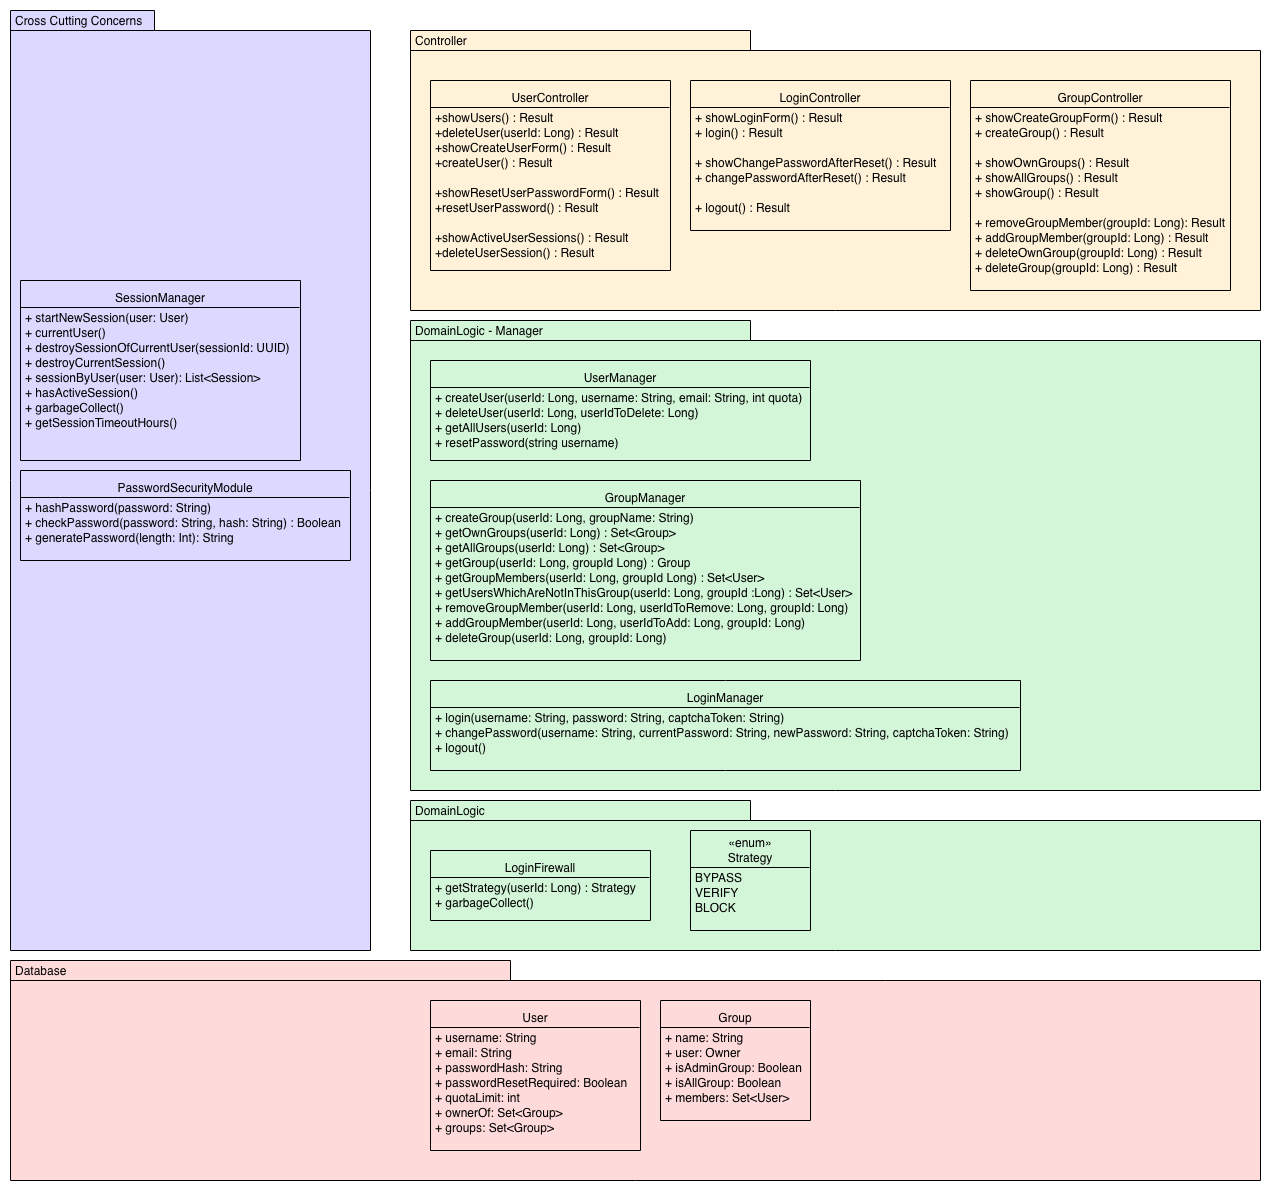
\includegraphics[width=0.93\paperwidth]{resources/class_diagram.png}
	\label{architecture:class_diagram}
\end{figure}

\chapter{\enquote{High-Level}-Klassendiagramm unseres Systems (Zweite Iteration)}
\begin{figure}[!htb]
\hspace*{-2.5cm}
	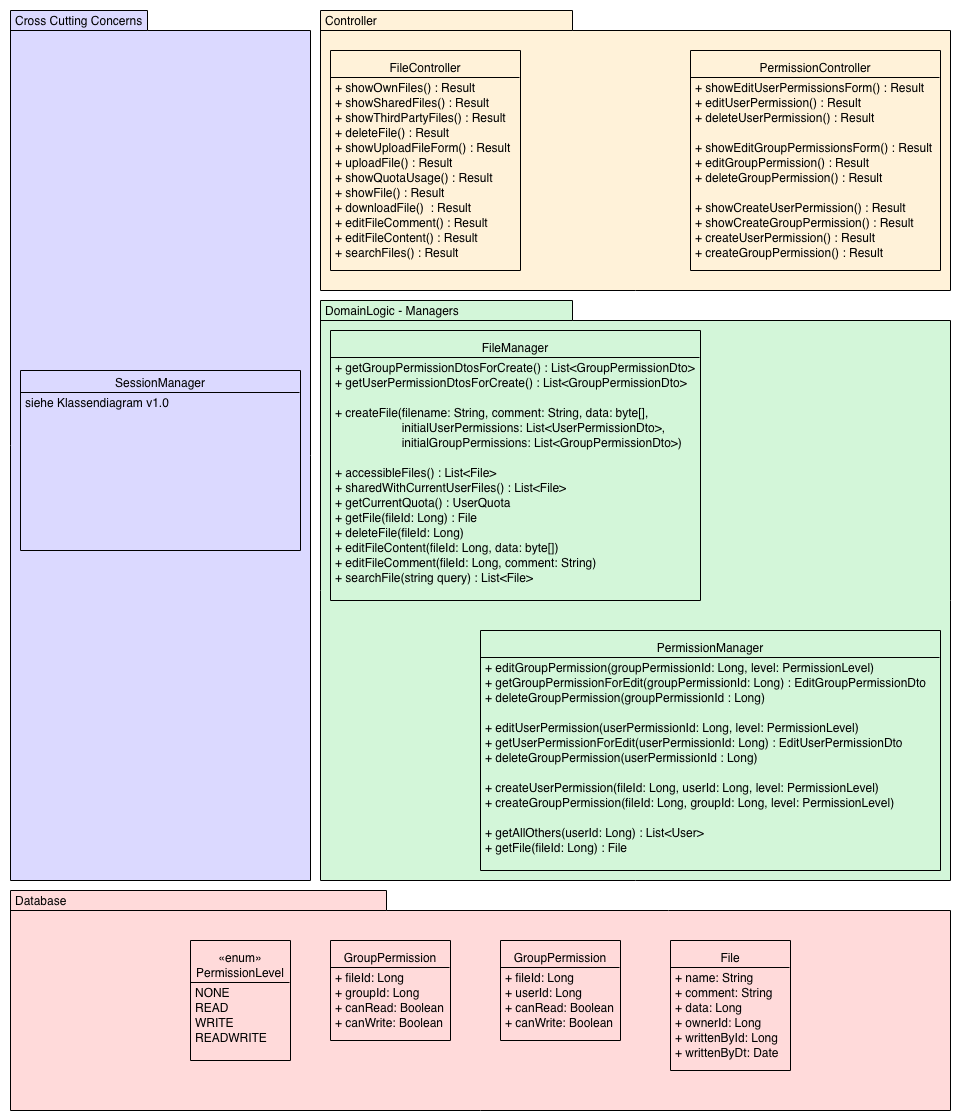
\includegraphics[width=0.93\paperwidth]{resources/class_diagram_2.png}
	\label{architecture:class_diagram2}
\end{figure}

\chapter{Sequenzdiagramm für \enquote{Benutzer erstellen}-Prozess}
\begin{figure}[!htb]
	\hspace*{-1cm}
	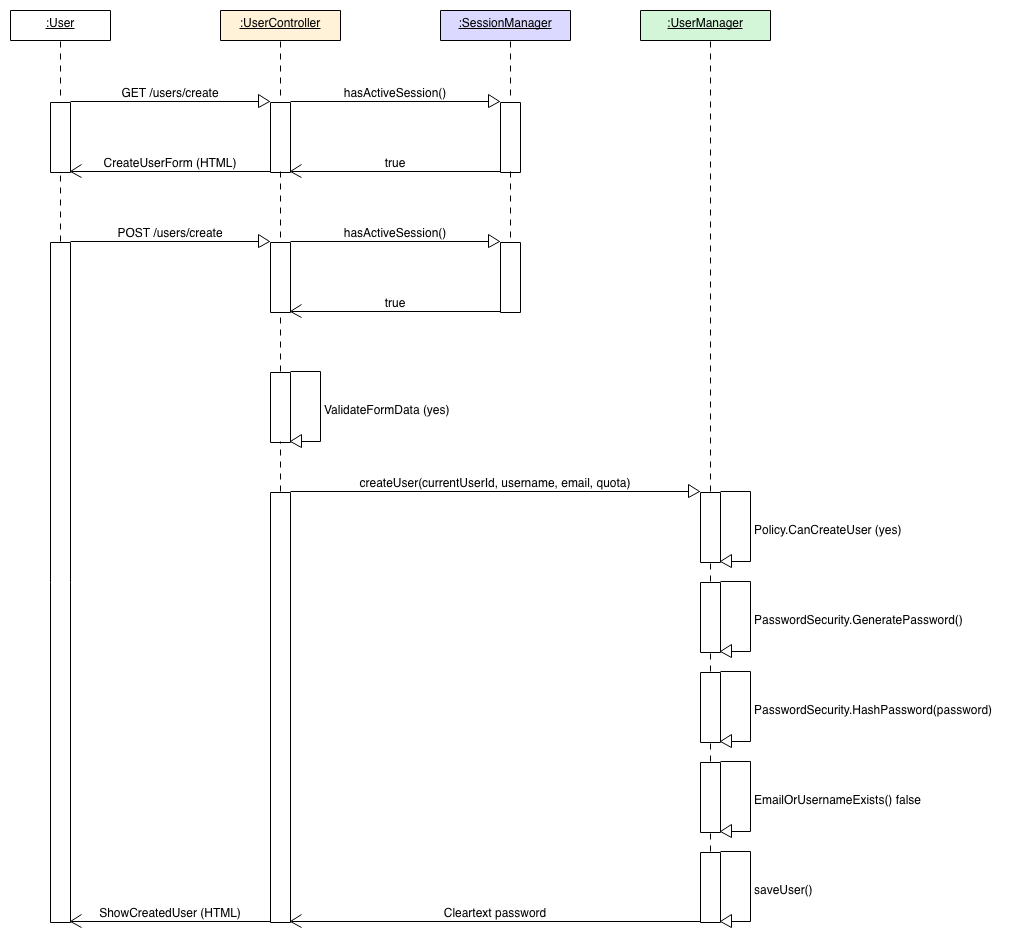
\includegraphics[width=0.83\paperwidth]{resources/createuserseq_diagram.png}
	\label{architecture:createuserseq_diagram}
\end{figure}

\chapter{Sequenzdiagramm für \enquote{Login}-Prozess}
\begin{figure}[!htb]
	\hspace*{-1cm}
	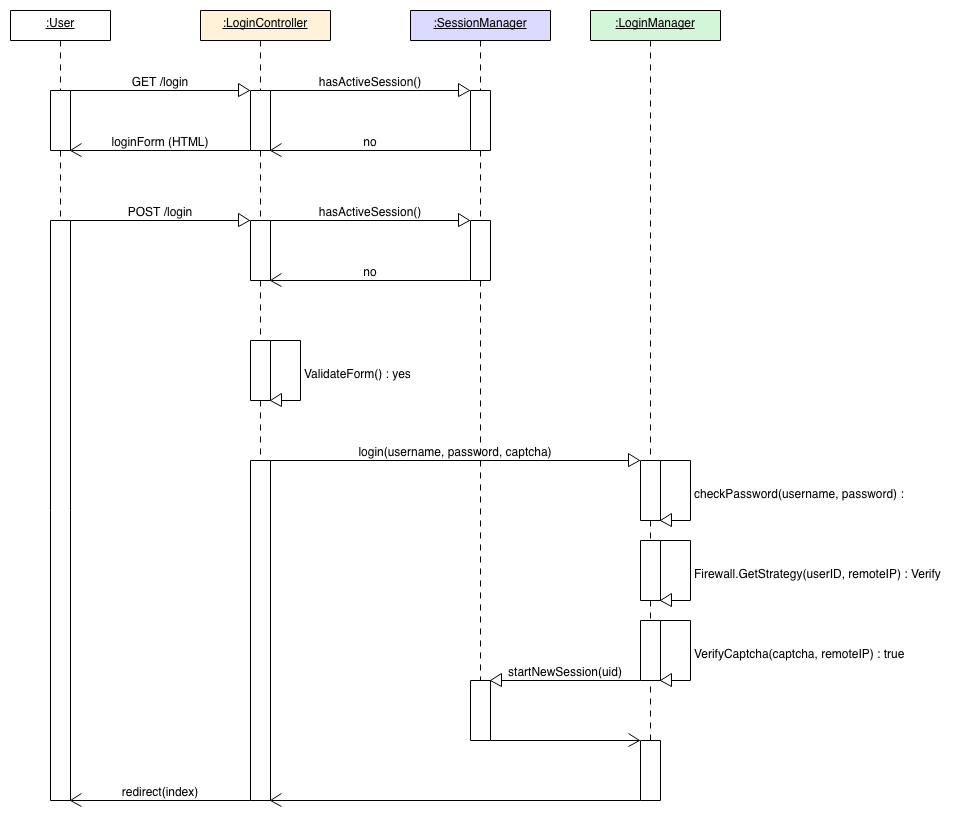
\includegraphics[width=0.83\paperwidth]{resources/loginseq_diagram.png}
	\label{architecture:loginseq_diagram}
\end{figure}

\end{appendices}

\end{document}
